\section{
    Effect of uniform relative motion on the Rheology at finite Reynolds number. 
    % phase relative velocity on the rheology of mono-disperse dilute emulsion of deformable droplets
    }
\label{sec:particle_def}






% \subsubsection{The zeroth simple laws}








Preceding studies have intended to model the rheology of dilute emulsion of neutrally buoyant deformable droplets, in stokes regime \citep{goddard1967nonlinear,lhuillier1987phenomenology,maffettone1998equation}.
More recently, researcher have been trying to include inertial effect in these models \citet{raja2010inertial,mwasame2018macroscopic}. 
However, these studies have been conducted in the objective of determining the response to mean shearing motion of a neutrally buoyant suspension on the stress, i.e. they study the mean stress $\bm{\sigma}$ in terms of the imposed flow gradient $\textbf{E}_f$ for a given microstructure. 
To the knowledge of the author all preceding study disregards the impact of relative motion, that we will not $\textbf{u}_{fp} = \textbf{u}_f - \textbf{u}_p$ on the suspension rheology.
We recall that $\textbf{u}_{p f} = \textbf{u}_p  - \textbf{u}_f$ is the relative averaged center of mass velocity of the droplet and the carrier fluid,  and $\textbf{E}_f$ is the fluid phase mean shear rate. 


Thus, in this section we make use of the \textit{hybrid model} derived in the preceding section to demonstrate what are the effect of uniform phase relative motion on the Rheology at finite Reynolds number. 
As this problem is rather complicated we firstly, state some simplifying hypothesis. 
We start by considering only uniform relative motion. 
Indeed, as the purpose is to point out the effect of the relative translational motions on the stress, we consider that there is no mean shear within the emulsion, i.e. $\textbf{E}_f = 0$. 
As discussed in the preceding section we consider that the droplet shape relax instantaneously, in other worlds we consider that the deformation of the drops are in quasi-steady state regime. 
Finally, as stated since the beginning of this chapter we only focus on small deformation.  



To introduce the problem we firstly introduce a way to compute analytically the droplet deformation in terms of its relative motion with the carrier phase. 
Indeed, it is shown with the help of the reciprocal theorem that closure term can be obtained at $\mathcal{O}(Re \phi)$, and therefore we obtain an explicit formula for the droplet deformation. 
We deduce from this application that at finite Reynolds number, the first moment of the hydrodynamic forces than was the cause of the droplet deformation acts also as a source term inside the mean carrier fluid stress. 
Thus, in a second step we expose a complete closed formulation of the bulk stress. 


The particle averaged linear momentum and mass conservation, can be obtained carrying exactly the same procedure as in \ref{chap:daniel1} and yield exactly the same as for non-deformable particles. 
Only the closure terms of the momentum equation will be influenced by the consideration of the drop shape and orientation.
Same comments can be done regarding the carrier phase equations. 
This implies that the equations used in \ref{chap:daniel1} are still valid upon having the right closure terms. 
Anyhow, for a mono-disperse suspension these equations provide an equation for the mean particle phase velocity $\textbf{u}_p$ fluid velocity $\textbf{u}_f$ and particle volume fraction $\phi$. 
Thus, in the closure problem these variables are considered as known variables. 

\subsection{Determination of the averaged particle shape}

In \ref{sec:local_eq_ellipse} we have seen that in the quasi-steady state regime the rate of strain equation, i.e. the equation for $\textbf{E}_\alpha$, becomes directly an equation for the particle shape. 
Indeed, applying the average operator on \ref{eq:steady} yields,
\begin{equation}
    (\bm\chi_{p})_{ij}
    = 
    \frac{5}{4}Ca \left[
        (\textbf{F}_p^h )_{ij}
        + \zeta Re (\textbf{F}_p^{vv})_{ij}
        +    \lambda (\textbf{F}_p^{\sigma})_{ij}
    \right],
    \label{eq:steady_state_avg}
\end{equation}
where we introduced, $n_p \textbf{F}_p^h = \pavg{\textbf{F}_\alpha^h}$ and so on. 
Thus, in this regime, one might be able to compute the instantaneous averaged shape of the particle upon the knowledge of the surface stress distribution, the particle internal shear and finally, the particle internal inertia. 

As the purpose of this section is to determine the effect of relative motion on the shape of the particles, we will consider only the portion of the closures that are functions of $\textbf{u}_{pf}$, which is the relative phase velocity. 

\subsubsection{Discussion on the closure problem}   

However, to broaden our understanding, we first propose to discus what form the right-hand side of \ref{eq:steady_state_avg} may take in the simplest scenario. 
Only for this subsection we consider a mean shear rate $\textbf{E}_f$ since it is useful for the subsequent discussion. 

Let us first discuss the term $\textbf{F}^{vv}$. 
It is clear that a complete closure for this term taking into account all parameters at hand is impossible. 
Nevertheless, as shown in \ref{ap:reciprocal} we may already compute this term assuming only the translation of a spherical droplet in stokes flow. 
As this term is inertial by nature, its computation from the stokes flow solution just gives us the first order in $Re$ accurate term.
Thus, for $Re \zeta < 1$, $Ca = 0$ and $\phi = 0$ we may write,
\begin{align}
    \textbf{F}^{vv}_p
    % &= 
    % \intO{\rho_d [\textbf{v}_d^0  \textbf{v}_d^0  - \frac{1}{3}\rho_d (\textbf{v}_d^0 \cdot \textbf{v}_d^0)\bm\delta]}\\
    = \frac{\rho_d \phi_d}{20(\lambda +1 )^2}
    \left[
        \textbf{u}_{p f}\textbf{u}_{p f} 
    -\frac{1}{3} (\textbf{u}_{p f}\cdot \textbf{u}_{p f})\bm\delta
    % + 7\pavg{\textbf{u}_\alpha'\textbf{u}_\alpha'}/n_p 
    % + 2k_p \bm\delta
    \right]
    + \frac{\rho_d \phi_d a^2}{21 (\lambda + 1)^2}[\textbf{E}_f\cdot \textbf{E}_f - \frac{1}{3}(\textbf{E}:\textbf{E})\bm\delta]
    + \mathcal{O}((Re\zeta)^2,Ca, \phi)
    \label{eq:vv_closure}
\end{align}
This closure is valid solely for spherical particles at first order in $Re$. 
Thus, as soon as the particle deform an additional correction must be provided to account for this deformation. 
Notice that these corrections can be obtained at low but finite capillary number $Ca$, from \citet{leal2007advanced} for a droplet immersed in a pure linear flows, and \citet{taylor1964deformation} for a droplet in relative translation. 
Anyhow, with the derivation of $\textbf{F}^{vv}$ we would like to point out that due to the presence of $\textbf{u}_{\alpha f}$ in \ref{eq:vv_closure} the internal droplets motions, $\textbf{v}_d^0$, induce a coupling between the droplets translational motion $\textbf{u}_\alpha$ and deformation $\bm\chi_\alpha$ through \ref{eq:dev_dim}. 
As it could be expected, the fluid phase shear rate $\textbf{E}_f$ also induce an internal motion (see \ref{fig:flowlines}), which when accounting for the particle inertia plays a role on the dynamical shape balance.  
To conclude, notice that $\textbf{F}^{vv}$ is the only reason why the density ratio $\zeta$ comes into plays when computing the steady-state shape of a droplet (for example see \citet{taylor1964deformation}). 

The internal particle shear rate forcing term $\textbf{F}^\sigma$, also plays an important role in the shape dynamics. 
Applying the previous reasoning we may have a first glimpse of the functional form of this term by using the Stokes flow singularity solution. 
Indeed, from \ref{ap:Translating_sphere} we found that, 
\begin{equation*}
    \textbf{F}_p^{\sigma}
    % = - \mu_d \intS{(\textbf{n}_i \textbf{v}_{d,j}^0 + \textbf{n}_j \textbf{v}_{d,i}^0)}
    = \mu_d \phi \frac{ 2 }{\lambda+1}
    \textbf{E}_f
    + \mathcal{O}(Re,Ca,\phi). 
\end{equation*}
In this situation notice the absence of $\textbf{u}_{\alpha f}$, this is due to the fact that the translation of a droplet in stokes flow do not alter the shape of the droplets, implying that this term is null at zeroth order in $Re$. 
Nevertheless, at $\mathcal{O}(Re^2)$ it is reasonable to expect the emergence of $\textbf{u}_{\alpha f}$.
Approximately the same treatment can be adopted for the external stress contribution $\textbf{F}^h$. 
Indeed, it is found that, 
\begin{equation*}
    % \pavg{\intS{\textbf{r}\bm{\sigma}_f^0 \cdot \textbf{n}_d}} 
    \textbf{F}^h_p
    = 
    \frac{3}{5}\mu_f \phi_d \left(\frac{2+5\lambda}{1+\lambda}\right)
    \textbf{E}_f
    + \mathcal{O}(Re,Ca,\phi).
\end{equation*}
Again at the next order in $Re$ it is likely that the translation of the droplet might contribute to this term. 
Introducing again a coupling between deformation and particle translation. 
Nevertheless, under this form the closure problem is incomplete as \ref{eq:dev} require to compute the closure term with an accuracy of $\mathcal{O}(Ca)$ at least. 
Notice that in \citet{raja2010inertial} they give the next order in $Ca$ for this term.
Anyhow, work remain to be done on this matter. 


Overall, we have shown that these closure terms can indeed be expressed as a combination of particles and carrier fluid properties.
Particularly, we demonstrated that there is an explicit link between deformation and translational velocity of the particle at finite $Re$. 
As observed here, these tensors equations are useful since their may be related to the fluid phase tensor unknowns in order to obtain an equation valid in the laboratory reference frame. 

Overall, we have shown that these closures could be expressed based on the singularity solution of stokes flows. 
It is clear that the relative velocity plays a role only at finite Reynolds number. 
Indeed, at $Re = 0$ only the mean fluid shear rate $\textbf{E}_f$ is present in the source term. 
Therefore, as our objective is to determine the effect of relative motion on the shape of the particle, we decide to compute the closure terms at $\mathcal{O}(Re)$ since it will eventually make appear the relation of these closures with the relative motion $\textbf{u}_{pf}$. 


\subsubsection{Determination of the closure terms at first order in $Re$}

We proceed and expand each closure terms in at Taylor expansion about $Re = 0$. 
We define, 
\begin{align*}
    \textbf{F}_p(Re)
    = 
    \textbf{F}_p^{(0)}
    + Re\textbf{F}_p^{(1)}
    + \ldots 
    = 
    [(\textbf{F}^h_p)^{(0)}+\lambda (\textbf{F}^\sigma_p)^{(0)}]
    + Re[(\textbf{F}^h_p)^{(1)}+\lambda (\textbf{F}^\sigma_p)^{(1)}+\zeta (\textbf{F}^{vv}_p)^{(0)}]
    + \ldots 
\end{align*}
where the terms with  superscript $^{(0)}$ correspond to the stokes flow solution and the ones with $^{(1)}$ to the first inertial correction. 
It is interesting to notice that to be accurate at the first order in $Re$ this requires to compute the term $(\textbf{F}^{vv}_p)^{(0)}$, which is the zeroth order inertial correction of the internal velocity circulation.
In other worlds this term is the integral of the particle internal velocity in stokes flow.  
As we are interested only in the particle relative translation we can already obtain this term and show that, 
\begin{equation*}
    (\textbf{F}^{vv}_p)^{(0)}
    % &= 
    % \intO{\rho_d [\textbf{v}_d^0  \textbf{v}_d^0  - \frac{1}{3}\rho_d (\textbf{v}_d^0 \cdot \textbf{v}_d^0)\bm\delta]}\\
    = \frac{1}{20(\lambda +1 )^2}
        [\textbf{u}_{p f}\textbf{u}_{p f} 
    -\frac{1}{3} (\textbf{u}_{p f}\cdot \textbf{u}_{p f})\bm\delta]. 
    % + 7\pavg{\textbf{u}_\alpha'\textbf{u}_\alpha'}/n_p 
    % + 2k_p \bm\delta
    \label{eq:closure_vv}
\end{equation*}
Regarding the term $(\textbf{F}^h_p)^{(1)}$ and $\lambda (\textbf{F}^\sigma_p)^{(1)}$, the calculation becomes way more complicated and require the use of asymptotic method. 

Based on an original proof given in \ref{ap:reciprocal} we demonstrate how to compute $(\textbf{F}^h_p)^{(1)}$ and $\lambda (\textbf{F}^\sigma_p)^{(1)}$. 
The method is based on the reciprocal theorem, for finite $Re$ and is not limited to the context presented here.
Particularly, we show how to compute the first order correction in $\mathcal{O}(Re)$ of these closure in an arbitrary flows, meaning that it is not limited to the relative translation.
We show that the computation of $(\textbf{F}^h_p)^{(1)}$, independently of $\lambda (\textbf{F}^\sigma_p)^{(1)}$ were not possible, however we could demonstrate  how to compute the sum of these terms. 
Namely, 
\begin{align}
    (\textbf{F}^h_p)^{(1)}  
    + \lambda (\textbf{F}^\sigma_p)^{(1)}
    &=
    - C_1
    [
        \textbf{u}_{pf}\textbf{u}_{pf} - \frac{1}{3}(\textbf{u}_{pf}\cdot \textbf{u}_{pf})\bm\delta 
    ]\\
    C_1 &=
    % \frac{345 \lambda^{3} + 928 \lambda^{2} + 856 \lambda + 272}{320 \left(\lambda + 1\right)^{3}}
    % + \frac{\zeta \left(12 \lambda + 13\right)}{20 \left(\lambda + 1\right)^{2}}
    \frac{57 \lambda^{3} + 192 \lambda^{2} + 216 \lambda + 80}{320 \left(\lambda + 1\right)^{3}}
    % \intS{\textbf{u}_f^{(1)}\cdot  \hat{\bm\sigma}_f \cdot \textbf{n}}
    % \intOf{\textbf{u}_f^{(0)}\cdot ( \div \hat{\bm\sigma}_f)}
    \label{eq:closure_sigma_e}
\end{align}
This, proves indirectly that the Stresslet on a drop in translation is not null at finite $Re$. 
This result is entirely original. 
Notice the apparition of the droplet density ratio in this expression. 
This arises because the inertial components of the particle internal stress involves the density of the particle. 
Thus, in dimensionless form this involves the density ratio $\zeta$.
Notice that this derivation is based on spherical droplets' solution. 
Thus, they are only accurate at $\mathcal{O}(|\bm\chi|)$. 


Using \ref{eq:closure_vv} and \ref{eq:closure_sigma_e} in  \ref{eq:steady_state_avg}, the deformation can be estimated at $\mathcal{O}(Re,Ca)$ and yields, 
\begin{align*}
    (\bm\chi_{p})_{ij}
    &= 
    \frac{5}{4}We \left[
        (\textbf{F}_p^h )_{ij}^{(1)}
        + \lambda (\textbf{F}_p^{\sigma})_{ij}^{(1)}
        + \zeta (\textbf{F}_p^{vv})_{ij}^{(0)}
    \right]
    + \mathcal{O}(Re^{3/2})\\
    &= We \beta [\textbf{u}_{pf}\textbf{u}_{pf} - \frac{1}{3}(\textbf{u}_{pf}\cdot \textbf{u}_{pf})\bm\delta ]
    + \mathcal{O}(Re^{3/2}),
\end{align*}
with, 
\begin{equation*}
    \beta = 
    - \frac{345 \lambda^{3} + 928 \lambda^{2} + 856 \lambda + 272}{256 \left(\lambda + 1\right)^{3}}
    - \frac{3 \zeta}{4 \left(\lambda + 1\right)} 
\end{equation*}
where we have introduced the \textit{Weber} number $We = Re \cdot Ca$. 
Notice that $\beta < 0$ $\forall \lambda,\zeta$, which means that the droplet will eventually deform into an oblate ellipsoid.
This conclusion align with \citet{taylor1964deformation} even if the coefficient $\beta$ corresponding to $2\zeta$ in their  study does not correspond exactly.   

Let us now discuss the physical implication of the droplet deformation. 
If the droplet deform, this ultimately means that the local forces at the above and below the droplet are stronger than the forces on the sides of the droplets. 
If the droplet phase experience such imbalance in forces, this means that the continuous phase experience an equal, but opposite in sign local forces. 
Consequently, the average carrier fluid phase stress will ultimately be modified by this kind of forces. 
Thus, in the next section we compute the role of the forces inducing the droplet deformation on the carrier phase stress. 

% \subsection{Determination of the bulk stress}

% Rhetorical studies are most of the time carried in the purpose of finding out the expression of the stress in terms of the mean fluid phase shear. 
% In other world one is trying to find out the \textit{bulk stress} response from a mean shearing motion. 
% As we did not consider a mean shear rate in this study, our objective is to determine the \textit{bulk stress} induced by relative translating motions between phases.  

% A first part of the awnser is provided by the expression of the second moments of the hydrodynamic forces, 
% which we now reads, 
% \begin{equation}
%     \pSavg{\textbf{rr}(\bm\sigma\cdot \textbf{n})}
%     \sim \textbf{u}_{pf} \bm\delta.
% \end{equation}
% Nevertheless, this expression could not be carrier to the next order in $Re$. 
% Therefore, to stay consistent we dismiss this term by considering a homogeneous suspension of droplets, in which case the inhomogeneous terms vanish.
% In this situation we may write the equivalent homogeneous \textit{bulk} stress as, 
% \begin{equation*}
%     \bm{\sigma}_m^\text{ed}
%     = 
%     \avg{\rho^0\textbf{u}_m'\textbf{u}'_m}
%     + \phi_fp_f\bm\delta
%     - 2\mu_f\textbf{e}  
%     + \pOavg{(\bm{\sigma}_d^0 - 2\mu_f \textbf{e}_d^0)}
%     % - \phi_d(\bm{\sigma}_d - 2\mu_f \textbf{e}_d)
%     + \pSavg{\bm\sigma_I^0}. 
%     \label{eq:bulk_stress_translating}
% \end{equation*} 
% Notice that since we only consider relative translation the term $2 \mu_f \textbf{e}$ usually present, doesn't appears. 
% As discussed in the preceding chapter $\avg{\rho^0\textbf{u}_m'\textbf{u}'_m}$ is the pseudo-turbulent stress. 

% The second term on the right-hand side of \ref{eq:bulk_stress_translating} represent the fluid phase pressure, it is considered as an unknown and therefore does not need to be reformulated. 
% The third term, represents the particle internal stresses, usually we use the first moment of momentum balance to reformulate this term as surface integral of the fluid phase stress. 
% Nevertheless, in this context as we know exactly the particle stress constitutive relation we may write, 
% \begin{equation*}
%     \pOavg{(\bm\sigma_{d,ij}^0 -2\mu_f \textbf{e}_{d,ij}^0)}
%     =
%     - \pOavg{p_d^0} \bm\delta_{ij}
%     +2 \mu_f (\lambda - 1) \phi_d \textbf{E}_{p,ij}
%     + \mu_f (\lambda - 1) \pSavg{(\textbf{n}_i \textbf{v}_{d,j}^0 + \textbf{n}_j \textbf{v}_{d,i}^0)}
%     % - \mu_f  \pSavg{(\textbf{n}_i \textbf{v}_{d,j}^0 + \textbf{n}_j \textbf{v}_{d,i}^0)}
% \end{equation*} 
% Then the last term of \ref{eq:bulk_stress_translating} is the surface tension stress which we see is expressible as, 
% \begin{equation*}
%     \pSavg{\bm\sigma_{I,ij}^0}
%     = \frac{\gamma \phi_d }{a} \left[
%         2\bm\delta_{ij} 
%         + \frac{4  }{5} \bm\chi_{p,ij}
%     \right]
% \end{equation*}
% Including all these expressions into the bulk stress leads to, 
% \begin{align*}
%     \bm{\sigma}_m^\text{ed}
%     = 
%     \avg{\rho^0\textbf{u}_m'\textbf{u}'_m}
%     + \left[
%         \phi_fp_f
%         - \pOavg{p_d^0}
%         +\frac{2 \gamma \phi_d }{a}
%     \right]\bm\delta
%     - 2\mu_f\textbf{e}
%     + 2 \mu_f (\lambda - 1) \phi_d \textbf{E}_{p,ij}\\
%     + \mu_f (\lambda - 1) \pSavg{(\textbf{n}_i \textbf{v}_{d,j}^0 + \textbf{n}_j \textbf{v}_{d,i}^0)}
%     % - \phi_d(\bm{\sigma}_d - 2\mu_f \textbf{e}_d)
%     +  \frac{4 \gamma \phi_d }{5 a} \bm\chi_{p,ij}
% \end{align*} 
% Notice that the terms within the bracts are all isotropic, meaning that they represent an effective pressure to the suspension, while the others terms are all symmetric traceless tensors. 
% Additionally, the presence of $\bm\chi_{p,ij}$ represents the elastic contribution of the particles. 
% In other worlds the suspension becomes visco-elastic in this regime. 
% To complete this expression one must solve \ref{eq:avg_chi_I} and \ref{eq:avg_E_I}, the orientation equations \eqref{eq:dt_Ap}. 
% Additionally, as the pressure of the particle phase appears explicitly in the equation, one may use \ref{eq:dt_trM2} which can be reformulated as, 
% \begin{equation*}
% % -  \bm\Gamma_{\alpha,ml}\bm\Gamma_{\alpha,mk} \textbf{M}_{\alpha,kl}  
% \frac{2\gamma \phi_d }{a} 
% - \pOavg{p_d^0} 
% = 
% \frac{1}{3}\pSavg{\textbf{r}_m\cdot\bm\sigma_{1,mk}^0\cdot \textbf{n}_k} 
% + \frac{1}{3}\pOavg{\rho_2 \textbf{v}_{d,m}^0\cdot \textbf{v}_{d,m}^0}. 
% \end{equation*}
% It is also possible to combine all these pressure term and solve for the sum of it. 


% \tb{Discus more this point on  a point of view phenomenological o not speak closures}
% \tb{make the link with the system of equation ? }


\subsection{The continuous phase stress}

The equivalent stress of the continuous phase momentum equations is now discussed. 
Particularly, notice that in 1D models the absence of mean shear is by definition assumed, therefore it is relevant to discuss the effect of relative translation on the mean continuous phase stress, since in this kind of situation this is the only contribution of the carrier phase stress. 

In the most general case the homogeneous averaged continuous phase stress can be written as, 
\begin{equation}
    \bm{\sigma}^\text{eq}_f = 
    \phi_f p_f \bm\delta 
    % - 2\mu_f \textbf{e} 
    +\avg{\rho_f\chi_f\textbf{u}_f'\textbf{u}_f'}
    % - \pSavg{\textbf{r}\times(\bm{\sigma}_f^0\cdot \textbf{n}_d)}
    % \\
    - \pSavg{\textbf{r}\bm{\sigma}_f^0\cdot \textbf{n}_d}
    + 2 \mu_f \pOavg{\textbf{e}_d^0}
    % \\
    % + \div \left[
    %     \frac{1}{2} \pSavg{\textbf{rr}\bm{\sigma}_f^0\cdot \textbf{n}_d}
    %     - 2 \mu_f\pOavg{ \textbf{re}_d^0 }
    %     + \ldots
    % \right]
    \label{eq:sigma_eq_f}
\end{equation} 
Again the mean shear rate $2\mu_f\textbf{e}$, usually present in this expression, does not appear since we are concerned with only relative motion and no macroscopic shear. 
Under this form it is clear that the mean carrier fluid stress is generated due to the competitive action of the mean continuous phase pressure, the \textit{Reynolds stress} tensor, and the \textit{Stresslet} tensor. 
As one can see the deformation of the droplets described by $\bm\chi_p$ as well as their rate of strain $\textbf{E}_p$ do not appear explicitly in the equivalent stress. 
However, that does not mean that they do not play a role in the averaged stress. 
Indeed, the exchange term in \ref{eq:sigma_eq_f} could be substituted using \ref{eq:dt_S} making appears explicitly those quantities witnessing of their importance. 
Nevertheless, as it has been shown, in the steady state regime we obtained algebraic expressions for $\bm\chi_p$ and neglected $\textbf{E}_p$. 
This, means that in this context we may rather directly find a closure for the \textit{Stresslet} and \textit{Reynolds stress} tensor in terms of the particles and carrier fluid properties. 
Since we only assume relative and uniform motion, closing \ref{eq:sigma_eq_f} means that we must find the relation of these closures with relative mean motion.

In the most general scenario one would solve an equation for $\textbf{u}_p$, $\textbf{u}_f$, $\bm\chi_p$, $\textbf{E}_p$ and, upon having the right closures, he would compute the stress based on this potential expression. 
In the limit of the dilute regime, meaning that we neglect all terms $\sim \mathcal{O}(\phi^2)$ or higher, and only considering relative translational motions, these closures can be determined. 
As we have shown the \textit{Reynolds stress} tensor can be entirely closed in the steady state homogeneous dilute regime and yields, 
\begin{equation}
    \avg{\rho_f\chi_f\textbf{u}_f'\textbf{u}'_f}
    = Re  \phi C_{Re}^1 \left[
        \textbf{u}_{pf}
        \textbf{u}_{pf}
        -\frac{1}{3}
        (\textbf{u}_{pf}
        \cdot\textbf{u}_{pf})\bm\delta
    \right]
    + Re \phi C_{Re}^2 (\textbf{u}_{pf}\cdot\textbf{u}_{pf}) \bm\delta, 
    \label{eq:Reynolds_stress}
\end{equation}
where, 
\begin{align*}
    C_{Re}^1(\phi,\lambda)
    = \frac{1}{20(1+l)^2}\left[
        \frac{9(2+3\lambda)^2}{4}\Gamma(1/3) \phi^{-1/3}
        - (27+82\lambda +62\lambda^2)
    \right],\\
    C_{Re}^2(\phi,\lambda)
    = \frac{1}{6(1+l)^2}\left[
        \frac{(2+3\lambda)^2}{4}\Gamma(1/3) \phi^{-1/3}
        - (3+10\lambda +8\lambda^2)
    \right],
\end{align*}
Notice that the constant $C_{Re}^2$ and $C_{Re}^1$ are still function of $\phi$ due to the non-linear relation of $\avg{\rho_f\chi_f\textbf{u}_f'\textbf{u}'_f}$ with the volume fraction. 
Also, notice that in opposition to the \textit{Stresslet} term, the \textit{Reynolds stress} doesn't involve the ratio of the density $\zeta$. 
Additionally, we have decomposed the right-hand side terms of \ref{eq:Reynolds_stress}, such that the first term, proportional to $C_{Re}^1$, corresponds to a traceless symmetric tensor, and the second term proportional to $C_{Re}^2$, represents the isotropic contribution.  

The \textit{Stresslet term} has been derived in \ref{ap:reciprocal}. 
It is shown that the zeroth order Reynolds number term is identically null. 
Indeed, a droplet in uniform and steady translation in stokes flow does not experience any deformation, it is at equilibrium in its spherical shape.
Therefore, as witnessed by \ref{eq:stokes_shape} the first moment of hydrodynamic force is necessarily null in this situation to preserve a state of equilibrium. 
As we have discussed above this is not the case when small inertial effects are considered, especially, at first order we have (see \ref{ap:reciprocal}),
\begin{equation*}
    \pSavg{\textbf{r}\bm{\sigma}_f^0 \cdot \textbf{n}_d}
    - 2 \mu_f \pOavg{\textbf{e}_d^0}
    =
    - \phi Re C_1
    [
        \textbf{u}_{pf}\textbf{u}_{pf} - \frac{1}{3}(\textbf{u}_{pf}\cdot \textbf{u}_{pf})\bm\delta 
    ]
    + Re \phi C_2 (\textbf{u}_{pf}\cdot \textbf{u}_{pf}) 
    + \phi p_f \bm\delta
    \label{eq:stresslet_trans}
\end{equation*} 
where the constant $C_1$ is shown to be exactly the same as in \ref{eq:closure_sigma_e} and the constant $C_2 =\frac{3\lambda^2 + 6\lambda + 4}{48(\lambda +1 )^2}$. 
In the same way as for the \textit{Reynolds stress} term we have decomposed the \textit{Stresslet} into an isotropic and symmetric traceless tensor, proportional to $C_2$ and $C_1$, respectively. 
Notice that this time, $C_1$ and $C_2$ are not function of the volume fraction, but in opposition to the \textit{Reynolds stress} they depend on the density ratio. 

Making use of \ref{eq:Reynolds_stress} and \ref{eq:stresslet_trans} inside \ref{eq:sigma_eq_f} yields the following formula for the carrier fluid averaged stress, 
\begin{multline*}
    \bm{\sigma}^\text{eq}_f = 
    \left[ p_f + Re \phi  [C_{Re}^2(\phi,\lambda) + C_2(\lambda,\zeta)](\textbf{u}_{pf}\cdot \textbf{u}_{pf}) \right]\bm\delta \\
    % - 2\mu_f \textbf{e} 
    % +\avg{\rho_f\chi_f\textbf{u}_f'\textbf{u}_f'} \\
    + Re \phi [C_{Re}^1(\phi,\lambda) + C_1(\lambda,\zeta)]\left[
            \textbf{u}_{pf}\textbf{u}_{pf}
            - \frac{1}{3}(\textbf{u}_{pf}\cdot \textbf{u}_{pf})\bm\delta
    \right]
    + \mathcal{O}(Re^{3/2},\phi^2, Ca^2 )
\end{multline*} 
We remark that the terms on the first line correspond to an equivalent pressure term formed of, 
(1) the mean carrier fluid hydrostatic pressure $p_f$. 
(2) the isotropic contribution of the \textit{Reynolds stress}, 
(3) and the isotropic part of the \textit{Stresslet}, both proportional to $Re \phi (\textbf{u}_{fp}\cdot \textbf{u}_{fp})$.  
The terms on the second line represent the effective symmetric and traceless part of the carrier phase stress. 
This term is entirely due to the particles motion. 



Overall, at steady state equilibrium and for uniform relative motion the stress is driven by two distrinct physical contribution: 
(1) the \textit{Reynolds stress}, also called the particle induced turbulence. 
(2) the \textit{Stresslet} tensor which is also proportional to these two parameters. 
Notice that the particle induced turbulence is well known term. 
Even though the closure provided here is new, many peopoles conducted studies to model this term in the case of relative motion between phases. 
The latter contribution is often taken in account when mean shearing motion are considered, especially this term is teh cause of the well known Einstein viscosity. 
However, the value of this term in the presence of relative phase velocity, see \ref{eq:stresslet_trans},  and a small amount of inertia have been completely overlooked in the literature. 
Therefore, the presence of this term in the stress constitutive equation is completely new and seems to have been ignored up to now. 
For these reasons we now evaluate the relative importance of the \textit{Reynolds stress} often used in this context compared to the \textit{Stresslet} term. 

\begin{figure}
    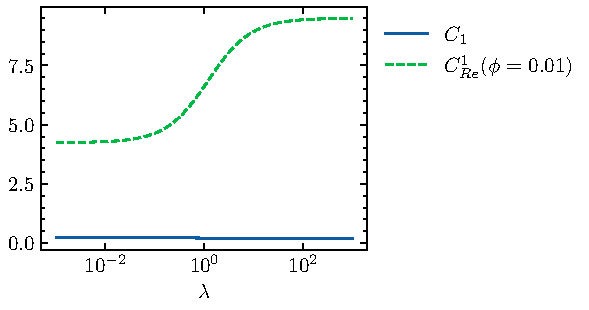
\includegraphics[height=0.25\textwidth]{image/Theory/C1.pdf}
    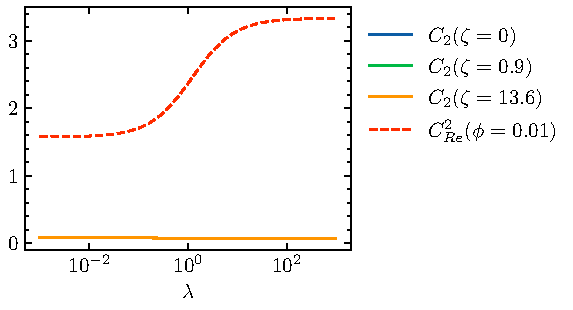
\includegraphics[height=0.25\textwidth]{image/Theory/C2.pdf}
    \caption{
    (solid lines) Values based on \ref{eq:stresslet_trans} of the constant $C_1$ (left)  and $C_2$ (right) for multiple density ratio $\zeta$ in terms of the viscosity ratio $\lambda$.
    (dashed lines) Values based on \ref{eq:Reynolds_stress} of the constant $C_1^{Re}$ (left) and $C_2^{Re}$ (right)  evaluated at $\phi = 0.01$ in terms of the viscosity ratio $\lambda$.
    }
    \label{fig:relative_comparaison}
\end{figure}
Since, $C_1^{Re} \& C_2^{Re} \sim \phi^{-1/3}$ we may already conclude that the $C_1^{Re} \ll C_1$ and $C_2^{Re} \ll C_2$ when $\phi \to 0$. 
This, means that for very low volume fraction the \textit{Stresslet} term  is in fact completely negligible. 
What about higher volume fraction ? 
Since our solution is derived in the dilute limit it seems reasonable to compare the values of the \textit{Reynolds stress} and the \textit{Stresslet} at a maximum value of $\phi = 0.01$. 
In \ref{fig:relative_comparaison} (right) we compare the isotropic contribution of the \textit{Stresslet} and \textit{Reynolds stress} at $\phi =0.01$. 
We can observe that the constant $C_{Re}^2 \ll C_2$ regardless of the density ratio $\zeta$. 
Consequently, the isotropic part of the \textit{Stresslet} due to relative translational motion might be entirely neglected. 
In \ref{fig:relative_comparaison} (left) we compare the symmetric traceless contribution of the \textit{Stresslet} for $\zeta = 13.6,0.9,0$ and \textit{Reynolds stress} at $\phi =0.01$. 
Before, doing so let us analysis the behavior of the \textit{Stresslet} in terms of $\zeta$ and $\lambda$ independently of the \textit{Reynolds stress}. 
These density ratios correspond to respectively, a drop of mercury in water $\zeta = 13.6$, a droplet of oil in water $\zeta = 0.9$ and a bubble in water $\zeta = 0$. 
We can observe on \ref{fig:relative_comparaison} (left) that $C_1(\zeta = 13.9)=C_1(\zeta = 0.9)=C_1(\zeta = 0)$ when $\lambda \to \infty$.
Consequently, in the low inertia regime the density ratio $\zeta$ doesn't impact the \textit{Stresslet} term. 
This is consistent with the quasi-steady state assumption adopted to derive these closures. 
At low $\lambda$ we observe that $C_1$ increases for the higher density ratios and decrease for the lower ones. 
Notice that a droplet of mercury in water has $\lambda =1$, thus this limit the realistic value that $C_1$ can take, i.e. a heavy droplet with $\lambda = 0$ might probably not exist. 
Now let us turns our attention to the \textit{Reynolds stress} contribution. 
We can observe as earlier on \ref{fig:relative_comparaison} (right) that $C_{Re}^1$ and $C_{Re}^2$ decrease for low viscosity ratio. 
This simply means that bubbles induce less velocity fluctuation than solid particle when being in steady translational motion in the fluid. 
This is easily explained by acknowledging that the fluid at the slip on the bubbles surface while it follows exactly the surface of a solid sphere, inducing more wakes. 
Therefore, as witnessed by \ref{fig:relative_comparaison} (left) the \textit{Stresslet} term is comparable, but still lower than the \textit{Reynolds stress} term.
The gap is lower for low $\lambda$ as the stresslet is in average higher and that the \textit{Reynolds stres} becomes less important. 
For high density ratio at $\lambda =1$ we can even identify that the \textit{Stresslet} becomes higher than the \textit{Reynolds stress}. 


Overall, we conclude that in this regime where the two competitive contribution to the mean carrier phase stress are the \textit{Reynolds stress} and the \textit{Stresslet} term, the latter cannot be neglect even tough being slightly lower than the former. 
Additionally, the isotropic part of the \textit{Stresslet} can however be safely neglected. 